\begin{frame}[t]{Self-driving cars react to traffic; software agents react to test results.}
\vspace{0pt}
\begin{columns}[T,onlytextwidth]
\column{.53\linewidth}
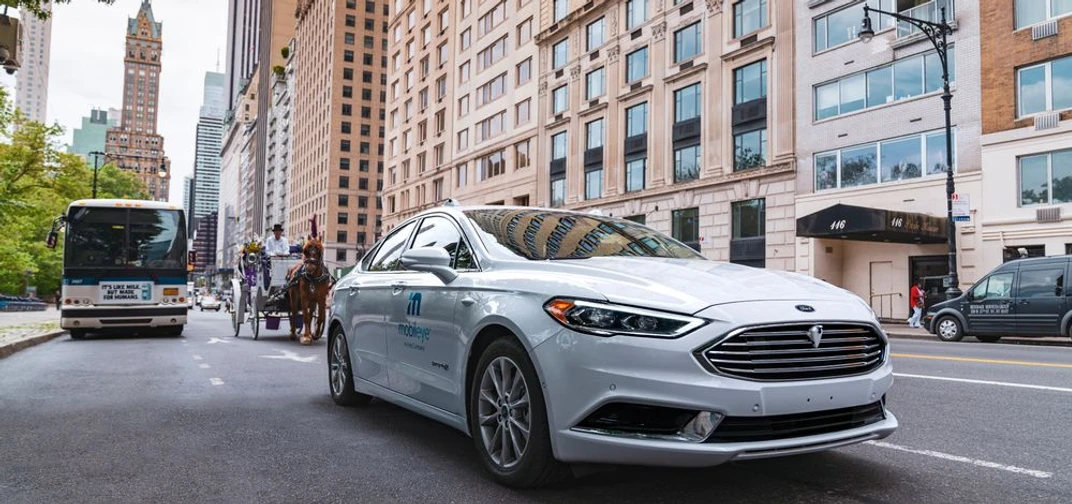
\includegraphics[width=\linewidth]{assets/mobileye-new-york-2021.png}\par
\vspace{.08cm}
\tagline{Mobileye test vehicle in Manhattan, June 2021.}
\column{.43\linewidth}
{\fontsize{12}{15}\selectfont
\textbf{Read the road.}\par
Find lanes, cars and pedestrians.\par
\vspace{.15cm}
A pedestrian steps out $\to$ brake $\to$ check the next camera frame.\par}
\vspace{.2cm}
\tagline{My work: junction perception at Mobileye, 2021--2024.}
\end{columns}
\vspace{.10cm}
\lead{\textbf{Software:} failing test $\to$ inspect code $\to$ edit $\to$ rerun the test.}
\sources{Photo: \href{https://www.mobileye.com/press-kit/press-kit-mobileye-new-york-city/}{Mobileye / Intel press kit}; Manhattan test drive, June 2021.}
\qadetail{The official Mobileye press kit identifies this photo as a test vehicle navigating Manhattan in June 2021. Image URL: https://static2.mobileye.com/img?h=504\&p=auto\&s=us\%2Fcorporate\%2Fimages\%2F17b6eecccb661bef7544a8bd66cc6a2c\_1668948799742.jpg\&w=1072. The vehicle illustrates the field; it is not attributed to the speaker's particular team or work. The speaker's own career website states Mobileye employment December 2021--March 2024, deep learning and algorithms research, including production perception and road-junction semantics. Perception provides observations for a driving policy; the pedestrian/braking sequence is an introductory illustration, not a description of a specific deployed Mobileye safety architecture or a personal contribution claim about the full controller. No Mobileye production accuracy or safety metric is asserted. The software loop is read an executed failure, inspect and edit the program, rerun the check, and revise. The proposed forkable execution layer adds private alternative continuations; ordinary stored-program execution still implements their actions. The downloaded WebP was converted losslessly to PNG for TeX compatibility, with no synthetic additions; it is scaled proportionally in the deck.}
\note{[0:35] At Mobileye I worked on junction perception. If a pedestrian steps into the road, perception detects it, the car brakes, and the next frame informs its next action. A software agent sees a failing test, edits the code and reruns the check. Both use feedback. A computer can also test several private alternatives before choosing one. That is the next step.}
\end{frame}
